\section {Assignment 1 \\ {Setup}}
\label {sec:assignment_1}

For this assignment we connected the Camera to the Virtual Machine. And to the project tempalte a case was addet to the "switch (key)" statement (see Listing \ref{lst:save_image}). This case was used to take a picture with the camera. The picture was then saved in the folder from wich the program was run.

\begin{lstlisting}[language=C, caption=save image to file, label=lst:save_image]
    case 's':
        cout << "Saving..." << endl;
        // save image using openCV API
        imwrite("blahai.png", image);
\end{lstlisting}

\begin{figure}[h!]
    \centering
    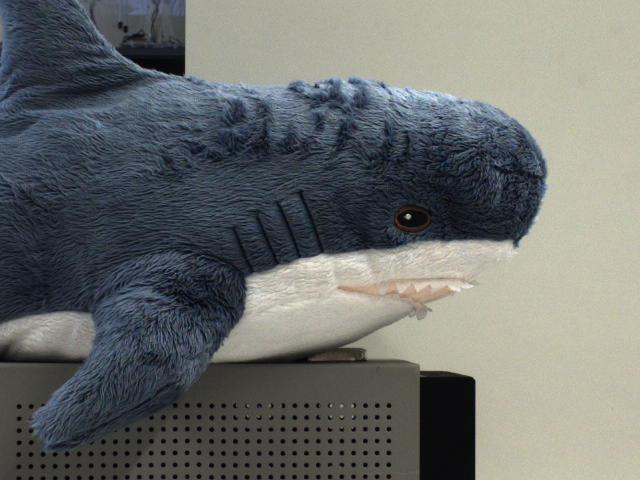
\includegraphics[width=0.5\textwidth]{blahai.png}
    \caption{Image taken with the camera of a blahai}
    \label{fig:blahai}
  \end{figure}

We pointed the camera at an object and adjusted the apature and focus to get a good looking picture with a shutter time of 100ms. See image \ref{fig:blahai}
